\section{Evaluation}
\label{sec:eval}

We ask two questions. Does memory help an agent answer questions about earlier
conversations, and what does each tier and each writer contribute (Section~\ref{sec:memory-eval})?
And how do the cache's replacement policies compare on an agent-shaped workload
(Section~\ref{sec:policy-eval})? Both benchmarks are synthetic and deterministic, and
need no language model. They show behaviour, not real-world accuracy.

\subsection{Does memory help?}
\label{sec:memory-eval}

\stitle{Workload.}
Twenty users chat with an assistant over 8, 32, or 64 sessions each. Facts come up in
passing; one is a request to remember (``Remember that my locker code is 4412'');
40\% of users move cities later; and the rest is chatter with distractors that look
like facts (``I like long walks'', ``My friend lives in Rome''). Half the statements
are in the forms the rule-based extractor is built for (``my dog is named Rex'') and
half are paraphrases it cannot parse (``Our dog goes by the name Rex''). Afterwards
each user is asked for their current city, their dog's name, their drink, and their
locker code. We report means over three seeds.

\stitle{Reader.}
A configuration builds a context for the question from its memory, and a
recency-aware reader answers from it: the answer is the latest-mentioned of the
values the user ever gave for the attribute, and it is right if that is the current
one. This measures what memory retrieves and how clean it is, not how well a model
reads.

\stitle{Configurations.}
\emph{Full history} gives the reader everything the user said. \emph{Episodic}
searches the record and returns the best three turns. \emph{Notes} are what dreaming
extracted with the rule-based extractor, searched and returned three at a time;
\emph{notes from tools only} are those the agent saved by tool call when asked to
remember. \emph{Episodic + notes} gives three items from each tier. The \emph{oracle}
variants replace the rule-based extractor with one that parses every phrasing the
workload uses: an upper bound on extraction, which a good model-backed extractor
would approach.

\begin{table}[t]
\caption{Accuracy by sessions per user, and words of context per question at 64
sessions. Starred rows use an oracle extractor (an upper bound).}
\label{tab:memory}
\small
\setlength{\tabcolsep}{4pt}
\begin{tabular}{lcccr}
\toprule
Configuration & 8 & 32 & 64 & Words \\
\midrule
none                         & 0.000 & 0.000 & 0.000 & 0 \\
full history                 & 1.000 & 1.000 & 1.000 & 1,358 \\
episodic search              & 0.958 & 0.958 & 0.958 & 20 \\
notes from tools only        & 0.154 & 0.133 & 0.113 & 3 \\
notes (rule extractor)       & 0.492 & 0.512 & 0.487 & 15 \\
episodic + notes             & 0.942 & 0.971 & 0.958 & 35 \\
notes (oracle)*              & 1.000 & 1.000 & 1.000 & 12 \\
episodic + notes (oracle)*   & 1.000 & 1.000 & 1.000 & 33 \\
\bottomrule
\end{tabular}
\end{table}

\begin{figure*}[t]
  \centering
  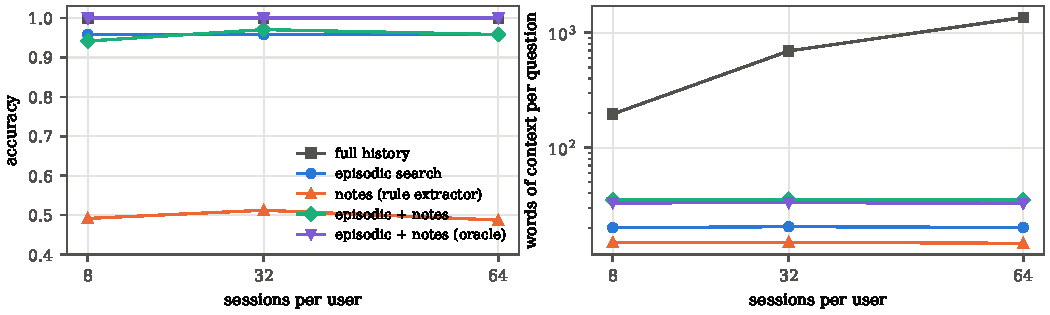
\includegraphics[width=0.8\textwidth]{fig/memory.pdf}
  \caption{Accuracy and context size as each user's history grows. The full history
  costs more with every session; search and notes read about the same amount at every
  length.}
  \label{fig:memory}
\end{figure*}

\stitle{Results.}
Table~\ref{tab:memory} and Figure~\ref{fig:memory} show four things.
(1)~\emph{The full history is not needed.} Search over the record reads about 20 words
where the full history needs 196, 694, and 1,358 as it grows, and is right 96\% of the
time.
(2)~\emph{Search alone fails on facts that change.} It is perfect on facts said once
(dog, drink, locker) and right on the city 83\% of the time, because a move often
shares few words with the question and the old statement is retrieved instead.
(3)~\emph{The notes fix that if extraction is good.} With a perfect extractor the
notes are right every time from 12 words, since the later statement supersedes the
old note and the reader sees one value. With the rule-based extractor, which parses
about half the phrasings, they are right about half the time, and the two tiers
together only match search alone. The extractor is the limit, not the pipeline.
(4)~\emph{Tools alone remember what they are told to.} Saving by tool call catches
the explicit request, and only when phrased as the agent is built to recognize it,
so accuracy is 0.11 to 0.15.

\stitle{Threats to validity.}
The workload is synthetic and small. Our first version stated every fact in the
phrasing the rule-based extractor is built for, and the notes scored 1.000; that was
circular, since both were written together, and the paraphrases are the correction.
The paraphrases were written to share a stem with the questions (``lived'' for
``live''), which favours lexical search; a paraphrase with no shared words would
defeat it and need an embedding index, which this benchmark does not test. Finally, a
recency-aware reader is not a language model.

\subsection{Eviction policies}
\label{sec:policy-eval}

We replay a synthetic agent-shaped workload (60 tasks writing 6 trace steps each,
then 472 skewed reuses of earlier memories) through the real store under each policy
and measure how often the memory an agent needs is still in working memory.
Table~\ref{tab:policy} shows hit rate at three capacities, and the log records the
policy cost at capacity 32. Every miss is a page-in and an eviction, both log records,
so cost follows quality: the forgetting curve has the best hit rate under the cap and
also writes the fewest records, 19\% fewer than FIFO. LFU and 2Q do poorly because
this workload reuses fresh trace steps often and both evict memories used only once
first. Which policy wins depends on the workload, which is why policies are pluggable
and the benchmark can replay one recorded from real agents.

\begin{table}[t]
\caption{Hit rate of working memory by capacity, and log records written at capacity 32.}
\label{tab:policy}
\small
\setlength{\tabcolsep}{4pt}
\begin{tabular}{lcccr}
\toprule
Policy & 16 & 32 & 64 & Records \\
\midrule
FIFO                & 0.506 & 0.551 & 0.602 & 1,112 \\
LRU                 & 0.642 & 0.744 & 0.828 & 930 \\
LFU                 & 0.354 & 0.460 & 0.606 & 1,198 \\
2Q                  & 0.381 & 0.481 & 0.606 & 1,178 \\
ARC                 & 0.551 & 0.663 & 0.763 & 1,006 \\
Forgetting curve    & \textbf{0.648} & \textbf{0.771} & \textbf{0.867} & \textbf{904} \\
Learned (logistic)  & 0.627 & 0.742 & 0.803 & 932 \\
\bottomrule
\end{tabular}
\end{table}
